\chapter{Real-Time scheduling and analysis}
In the previous chapter the reader was introduced to some fundamental notions and concepts that will be extensively used throughout the course.

Since, in this chapter, we will focus on the scheduling of real-time tasks and the analysis of each scheduling policy, it is worth mentioning some basic definitions:
\begin{itemize}
\item{\makebox[2cm]{Algorithm\hfill}logical procedure used to solve a problem}
\item{\makebox[2cm]{Program\hfill}formal description of an algorithm, using a programming language}
\item{\makebox[2cm]{Process\hfill}Instance of a program (program in execution)}
\begin{itemize}
\item Program: \side{static entity}
\item Process: \side{dynamic entity}
\end{itemize}
\item the term task is used to indicate a schedulable entity (either a process or a thread), in particular;
\begin{itemize}
\item A thread reresents a flow of execution (it executes with shared resources, multi thread within the same process)
\item A process represents a flow of execution + private resources (it executes with its own resources), such as address space, file table, etc...
\end{itemize}
\end{itemize}

Tasks do not run on bare hardware, but then how can multiple tasks execute on one single CPU?
The \side{OS kernel} is a piece of the operating system that takes care of multi-programming and somehow it is able to create the illusion that each CPU/processor has its own space, whereas in fact it is sharing the same resources with other processes.

In the end the kernel provides the mechanism that enable multiple tasks to execute in parallel; in a sense tasks have the illusion of executing concurrently on a dedicated CPU per task.

On this regard, with the term concurrency we refer to the simultaneous execution of multiple threads/processes in the same PC. 
\side{Concurrency} is implemented by \side{multiplexing} tasks on the same CPU. Tasks are alternated on a real CPU and the \side{task scheduler} decides which task executes at a given instant in time. In other terms, in order to implement the concurrency mechanism it is necessary to introduce this new component (i.e. the task scheduler), since it makes sure that the time of your pc is shared between the different processes or tasks that compete for the resources at that time.

Tasks are associated to temporal constraints (aka deadlines), hence the scheduler must allocate the CPU to tasks so that their deadlines are respected.

\section{Real-Time Scheduling}

One of the key components of an OS and a OS kernel is the scheduler.
A scheduler generates a schedule from a set of tasks. From a mathematical perspective it is a function:

first consider UP systems (given that it has a simpler definition).
A schedule $\sigma(t)$ is a function mapping (every point in) time $t$ into an executing task
\[\sigma : t\,\to\, \mathcal{T} \cup \tau_{idle}\]
where $\mathcal{T}$ os the \side{taskset} and $\tau_{idle}$ is the \side{idle task}.

At the end of the day what the processor/OS kernel does is to implement a function like the scheduler. Clearly, if you have more that one processor, the function under consideration is multivalued, because at every point in time it decide the allocation of the different processors to different tasks.\\
For an SMP system (i.e. $m$ CPUs), $\sigma(t)$ can be extended to map $t$ in vectors $\tau \in (\mathcal{T}\cup \tau_{idle})^m$.

Therefore, formally, the scheduler implements $\sigma(t)$ and as a consequence the scheduler is responsible for selecting the task to execute at time $t$. However, a function is a \side{denotational} way of describing an algorithm, i.e. we specify mathematically what the function is. The \side{operational} way of describing an algorithm on the other hand, is a squence of steps to be taken in order to implement the function.
 
Hence, from an operational/algorithmic point of view:
\begin{itemize}
\item \side{Scheduling algorithm} is an algorithm used to select for each time instant $t$ a task to be executed on a CPU among the ready task
\item Given a task set $\mathcal{T}$, a scheduling algorithm $\mathcal{A}$ generates the schedule $\sigma_{\mathcal{A}}(t)$
\end{itemize} 

In the frame of reference of real-time systems we are interested in finding conditions on the scheduling choice that allow us to meet all the deadlines. Hence, a task set is schedulable by an algorithm $\mathcal{A}$, if by applying that scheduling algorithm, $\sigma_{A}$ does not contain missed deadlines. 

On this note, the \side{Schedulability test} is a way to decide if, given a task set $\mathcal{T}$ and an algorithm $\mathcal{A}$, that task set is going to be schedulable.

The key point here is that given the fact that by making a proper choice of scheduling algorithm, one can obtain a schedulable task set, how can I find a way to schedule the activities so that all the deadlines are met? And this is the problem of real time scheduling.

\section{Cyclic Executive Scheduling}
One way to find a solution of the schedulability problem is to consider a task set of fixed tasks (i.e. you will always have those tasks activated in the very same way).
This is the case of legacy applications and where reliability is fundamental, e.g. military and avionics systems (Air traffic control, Space Shuttle, Boeing 777).

In this scenario, one can obtain a paper and pencil solution, i.e. trying to decide how to schedule things in such a way that the task set is schedulable and stick to that solution.

Of course, there is a more systematic way of solving such problem and such process is called \side{Cyclic Executive Scheduling}.\\
The Cyclic Executive Scheduling (aka \side{timelice scheduling} or \side{cyclic scheduling}) is a scheduling algorithm with very low overhead (in the sense that scheduling decisions are taken-offline) and with a very simple and well tested idea, that was originally used in avionic systems to schedule periodic tasks.

\subsection{The Idea}
Cyclic Executive Scheduling is a
\begin{itemize} 
\item \side{static scheduling algorithm} (i.e. it is decided offline and it is always applied repeatedly in the same way). 

As a consequence, all scheduling decision are taken upfront; it is not something that defers decision to the runtime. 
\item Jobs are assumed not to be preemptable, i.e. a scheduled job executes until termination, it retains control of the CPU for the entire computation time.
\end{itemize}
The procedure to follow in order to apply this scheduling algorithm is:
\begin{enumerate}
\item Split the time axis into slots, each of which is statically allocated to the tasks (\side{scheduling table}).
\item Since we are dealing with periodic tasks, the same sequence of tasks will repeat periodically, hence once the scheduling table is completed, it starts from the beginning and repeats the same sequence over and over again.
\end{enumerate}

A periodic timer activates execution (\side{allocation of a slot}).

In summary three components are needed to uniquely define this scheduling algorithm:
\begin{enumerate}
\item \side{Major Cycle}: least common multiple (lcm) of all the tasks' periods (aka \side{hyperperiod})
\item \side{Minor Cycle}: greatest common divison (gcd) of all the tasks' periods (i.e. granularity at which the scheduling decisions will repeat)
\item \side{A timer}: that fires every Minor Cycle ($\Delta$)
\end{enumerate}

\subsection{Implementation}
As previously mentioned from an execution stand point this scheduling algorithm is extremely simple because every minor cycle:
\begin{enumerate}
\item A periodic timer is initialized
\item Every time the timer fires the scheduler read the scheduling table
\item The scheduler calls the approriate function(s) associated to the corresponding task(s)
\item The scheduler returns to sleep until the next minor cycle (i.e. the timer fires)
\end{enumerate}

\subsection{Advantages}
From it's radical simplicity, allows to create a total check and a certification of the code that can be shipped to a space shuttle or any other avionic application and execute theoretically forever.

An OS is much more difficult to certify, because asynchronious events can be generated and it is impossible to consider upfront every possible course of events that can happen. On the contrary, once you solved the cyclic executing scheduling problem, you have a global solution that is guaranteed to be replicated.

Furthermore, with its simple implementation there is no need for a real-time operating system, no real task exist (just function calls), and only one single stack is necessary for all the \emph{tasks} (since each task runs until completion, there will never be a situation in which the execution of the function are active at the same time).

Since it involves a \side{non-preemptable scheduling} there is no critical races (i.e. there will never be two tasks that shared a variable) and therefore there is no need to protect data (i.e. no need for semaphores, pipes, mutexes, mailboxes, etc...).

Lastly, since there is no need for an OS, all the CPU/execution time is taken by the tasks, hence It has low run-time overhead, and the \side{jitter} (delay in which the result is completed, i.e. difference between when a task start and it finishes ) can be explicitly controlled.
\subsection{Drawbacks}

However, this scheduling algorithm has some important drawbacks:
\begin{itemize}
\item it is not robust w.r.t. overloads. This type of solution assumes that all the tasks do not give back control until they are finished (until its allocated slots terminates). However, if the task execute for much more of its WCET or the allocated time slot, what happens is that the schedule gets disrupted with a subsequent domino effect.
\item It is difficult to expand the schedule (static schedule): introducing a new task requires that the whole system/schedule must be redesigned.
\item Not easy to handle aperiodic/sporadic tasks
\item All task periods must be a multiple of the minor cycle time
\item Difficult to incorporate processes with long periods (big tables)
\item Variable computation time imply that it might be necessary to split tasks into a fixed number of fixed size procedures. This requires to actively change the code into smaller parts, and, in the case of third party library/code, this is not always allowed.
\end{itemize}

\section{Fixed Priority Scheduling}

In general, we want to have more flexibility than the cyclic executive scheduling (in fact it is applied on very niche and particular situations).

What can be done therefore is utilize \side{preemptive scheduling algorithm}s, i.e. algorithm that are allowed to suspend the execution of a task and resume it later.

Therefore a task has, two states: \side{ready} and \side{executing}, and the OS is allowed to enforce a state change.

In the class of preemptive algorithm we will look at different algorithms, but the simplest is the \side{Fixed Priority Scheduling}. In this scheduling algorithm:
\begin{itemize}
\item Every task $\tau_i$, when it is created, is assigned a integer number that is encoding a fixed priority $p_i$
\item The active task with the highest priority is scheduled (POSIX convention)
\end{itemize}
Priorities are integer numbers: the higher the number, the higher the priority (In the research literature, sometimes authors use the opposite convention).

And so, the work of the scheduler at any point in time is to look at the ready queue and pick up the task with the highest priority.

Observations:
\begin{itemize}
\item The response time of the task with the highest priority depends only on its computation time, and therefore it is always less than or equal to its WCET.
\item The response time of tasks with lower priority depends on its own computation time and the \side{interference} of higher priority tasks.
\item Clearly, the scheduling priorities can change how the things behave: are we sure that choosing a different priority assignment policy we would obtain a schedulable task set? Yes.

So, we have two issues: the \side{scheduling analysis} (given a task set and the priorities, is everything schedulable) and \side{syntesis problem} (given the task set and computation time, find the assignment of priorities that guarantees schedulability).
\end{itemize}

\subsection{Priority Assignment}
Given a task set how to assign priorities?\\
Depends on the different objectives that you would like to achieve:
\begin{itemize}
\item \side{Schedulability}, i.e. find the priority assignment that makes all tasks schedulable
\item \side{Response time (optimization)}, i.e. find the priority assignment that minimise the response time of a subset of tasks
\end{itemize}
By now we consider the first objective only, hence we will investigate the \side{optimal priority assignment (Opt)}.

\subsection{Optimal Priority Assignment}

A priority assignment is an optimal priority assignment (Opt):
\begin{itemize}
\item If the task set is schedulable with another priority assignment, then it is schedulable with priority assignment Opt (i.e. the optimal priority assignment cannot do any worse that any other feasible assignment).
\item If the task set is not schedulable with Opt, then it is not schedulable by any other assignment. (If the optimal choice fails then there is no other possible solutions/other alternatives will fail as well).
\end{itemize}

Formally, given a periodic task set $\mathcal{T}$ (all tasks are activated periodically) with all tasks having relative deadline $D_i$ equal to the period $T_i$ ($\forall i, D_i = T_i$), and with all offsets equal to 0 ($\forall i, r_{i,0} = 0$):
\begin{itemize}
\item The best assignment, in this case, is the \side{Rate Monotonic (RM)} assignment
\item Shorter period imply higher priority (hence the name rate monotonic: the priority is monotonic w.r.t. the rate. The higher the frequency/rate, the shorter the period, the higher the priority).
\end{itemize}

Given a periodic task set with deadline different from periods and with all offsets equal to 0 ($\forall i, r_{i,0} = 0$)
\begin{itemize}
\item The best assignment is the \side{Deadline Monotonic (DM)} assignment
\item Shorter relative deadline imply higher priority (the shorter the relative deadline, the higher the priority).
\end{itemize}
Note that the Deadline Monotonic assignment refers to relative deadline (interval in time, fixed value) not absolute deadline (instant in time, change over time).

For sporadic tasks, the same rules are valid as for periodic tasks with offsets equal to  and by considering maximum activation rate.

\section{Analysis}
The best possible assignment for fixed prority is the Rate Monotonic and Deadline Monotonic assignement.\\
But how can I be sure that even using the optimal priority assignment, the schedule will meet all the deadlines?

This is the problem of \side{Real-Time analysis}: an activity that given a task set  and a scheduling policy, it responds to the query on whether or not the task set is schedulable.

What we have done so far is something very naive, i.e. simulating the schedule and verify that there is no deadline miss, but does not scale well in the case of long observation time of the system, until the schedule repeats itself. \\
Luckly there is a point/tme horizon, such that if no deadline miss happens withing this time horizon, you can certify none will occur ever after. How long is this time horizon depends:
\begin{itemize}
\item If there is no offset, we will find ourselves in the critical case, because if we have simultaneous activation of all the tasks in the task set, the system have an immediate request of computation time that needs to be satisfied.

In this case, it is sufficient  to simulate the schedule until the \side{hyperperiod}, i.e. the least common multiple of the periods
\[H = lcm\{T_i\}\]
This is because after the least common multiple of the period the task activation will be repeated.
\item If there is an offset, the schedule diagram can be shifted to meet the condition of the previous point.

Anyhow, given an offset
\[\phi_i = r_{i,}\]
it is necessary to simulate the schedule for at least 
\[2\,H + \phi_{max}\]
before being sure that the schedule will repeat itself.
\item If tasks periods are prime numbers the hyperperiod can be very large
\end{itemize}

Fortunately, there are better tests, that we can find, called \side{Utilisation Bound Analysis}.

\subsection{Utilisation-Based Analysis}
The Utilisation is the fraction of the processor that a task needs for its execution.

Hence, if a task have an activation time of $5$ and a computation time of 1, then its utilization is around $\sfrac{1/5}  = 20\%$.

So it would be nice to have a test that tells if a scheduling algorithm produces as feasible schedule simply based, on the utilisation bound.

A sufficient test  is based on the \side{Utilisation bound}:

The \side{utilisation least upper bound} for scheduling algorithm $\mathcal{A}$ is the smallest possible utilisation $U_{lub}$ such that, for any task set $\mathcal{T}$, if the task set's utilisation $U$ is not greater than $U_{lub}$ ($U\le U_{lub}$), then the task set is schedulable by algorithm $\mathcal{A}$

Formally:
\begin{itemize}
\item Each task uses the processor for a fraction of time, called worst case utilisation
\[U_i = \cfrac{C_i}{T_i}\]
\item The total processor utilisation is 
\[ U = \sum_i \,\cfrac{C_i}{T_i}\]
and it is a measure of the processor's load
\end{itemize}

One thing that we can immediately say is that if the total utiilisation exceed 100 \% there is no way that the task set is schedulable, i.e.
\[U > 1\qquad\text{taskset is not schedulable}\]
If the sum of all the utilisation is greater than 1/100\% we encounter a situation called stochastic instability, meaning that in the average you are asking the system more than it can offer.

In this case we have something similar since we have the worst case utilisation. In case the system requires more that it is available, there is no way the taskset is schedulable. Hence, this analysis yield a worst case guarantee.

Moreover, if $U < U_{lub}$ the taskset is schedulable. However:
\begin{itemize}
\item there is a ``gray area'' between $U_{lub}$ and 1, it depends on the specific performance of the algorithm under consideration.

So the ability of an algorithm to achieve a good utilisation bound is a measure of how efficient and effective the algorithm is.
\item We would like to have $U_{lub}$ close to 1.
\item $U_{lub} = 1$ would be optimal (hard upper bound, after 1 we are sure that the task set is not schedulable), it is physical impossible to outperform 100\% utilisation.
\end{itemize}

\subsubsection{Utilisation Bound for RM}
The notion of least upper bound can be described considering 2 tasks: one can make many choices of periods and computation times of the two tasks, taking the minimum value of $U$ below which all the task sets that I can choose are schedulable.\\
It can happen that some task that exceed the $U_{lub}$ is schedulable, but following the notion of least upper bound, as far as the task set is below this value the task set is guaranteed to be schedulable.

Formally: consider $n$ periodic (or sporadic) tasks with relative deadline equal to periods. The least upper bound for Rate Monotonic assignment can be obtained via the following expression:
\[U_{lub} = n(2^{\sfrac{1}{n}} - 1)\]
Note:
\begin{itemize}
\item $U_{lub}$ is a decreasing function of $n$
\item For large $n$: $U_{lub}\approx 0.69$
\end{itemize}

\begin{table}[!h]
\centering
\begin{NiceTabular}[hvlines]{c|c||c|c}
$\mathbf{n}$&$\mathbf{U}_{lub}$&$\mathbf{n}$&$\mathbf{U}_{lub}$\\
2 & 0.828 & 7&0.728\\
3 & 0.779 & 8 & 0.724\\
4 & 0.756 & 9 &0.720\\
5 & 0.743 & 10 & 0.717\\
6 & 0.734 & 11 & ...\\
\end{NiceTabular}
\end{table}

Therefore the schedulability test consists in:
\begin{enumerate}
\item Computing the utilisation
\[U = \sum_{i=1}^{n} \cfrac{C_i}{T_i}\]
\item If $U \le U_{lub}$, the task set is schedulable
\item If $U > 1$ the task set is not schedulable
\item If $U_{lub} < U \le 1$, the task set may or may not be schedulable
\end{enumerate}

\subsubsection{Utilisation Bound for DM}
In case of deadlines different from periods, one can always consider a conservative approximation in which the period is equal to the deadline. 

If relative deadlines are less than or equal to periods, instead of considering 
\[U = \sum_{i=1}^n \cfrac{C_i}{T_i}\]
we can consider:
\[U' = \sum_{i=1}^n \cfrac{C_i}{D_i}\]
Then the test is the same as the one for RM, except that we must use $U'$, instead of $U$.

And consequently:
\[\tau = (C,D,T)\,\rightarrow\,\tau' = (C,D,D)\]
If I can guarantee that this conservative approximation is schedulable than I can guarantee that the original task set is schedulable as well.

In summary:
\begin{itemize}
\item $\tau'$ is a \emph{worst case} for $\tau$
\item If $\tau'$ can be guaranteed, $\tau$ can be guaranteed too
\end{itemize}

\subsubsection{Pessimism}

The previously described condition is an extremely conservative approximation and most often than not the test would yield a non-schedulable result (above the least upper bound, even though the task set is schedulable).\\
The bound is very pessimistic: most of the times, a task set with $U > U_{lub}$ is schedulable by RM.

A particular case is when tasks have periods that are \side{harmonic}: a task set is harmonic, if for every two tasks $\tau_i, \tau_j$ either $T_i$ is multiple of $T_j$ or $T_j$ is multiple of $T_i$. In this case, and only in this case, the least upper bound of RM grows to1 (i.e. For a harmonic task set, the utilization bound is $U_{lub} = 1$).

In other words, Rate Monotonic is an optimal algorithm for harmonic task sets.

\subsection{Response Time Analysis}
So far with the utilisation bound we have seen that there is a sufficient schedulability condition: if the total utilisation is below the least upper bound than the system is schedulable. But this test works only if one makes very specific choices, i.e. to have the priority set using the RM assignment, otherwise the least upper bound does not apply.\\
Moreover, in the case in which the total utilisation is above the least upper bound, no conclusion can be drawn/no guarantees.

Therefore, we would like to utilize a \side{necessary and sufficient} test, which won't be analytical and nice as we have seen from an algorithmic point of view, but it will be a little more reliable since it requires to make much less assumptions.

Before introducing this test, let us recall the concept of response time: difference between the activation and the finishing/completion time. If one is able to compute the \side{worst-case response time} and if one can verify that such quantity remains below the \side{relative deadline}, then the system is schedulable.

The best thing about this test is that there is no assumption on the priority assignment, hence it can be applied to all algorithms. However, the periodic or sporadic tasks that we will be consider, are assumed to have no offsets (even though it is possible to have a variant of this analysis that applies).

Formally:
\begin{itemize}
\item For every task $\tau_i$ in the task set
\item Compute the worst case response time $R_i$ for $\tau_i$, i.e.
\[R_i = \max_j\{\rho_{i,j}\}\quad\text{with:}\,\,\rho_{i,j} = f_{i,j} - r_{i,j}\]
\item If $R_i \le D_i$, then the task is schedulable
\item Otherwise, the task is not schedulable
\end{itemize}

Consider a number of task set ordered by decreasing priority (i.e. $i < j \rightarrow p_i > p_j$) and consider no assumptions about the tasks offset (i.e. tasks can be activated at any time). We can define the \side{Critical Instant} as the most critical condition for the computation of the response time (if you allow the offset to change).

The obvious result is that if you allow the offset to change, the worst case situation in terms of response time (i.e. situation that produces the longest response time) is one in which all tasks start at the same time. Because if all the tasks start at the same time one would observe an utilisation peak.

Consider:
\begin{itemize}
\item a number of task set ordered by decreasing priority (i.e. $i < j\rightarrow p_i > p_j$) 
\item no assumptions about the tasks offset (i.e. tasks can be activated at any time)
\item the worst possible offsets combination
\end{itemize}

A job $J_{i,j}$ released at the \side{critical instant} experiences the maximum response time for $\tau_i$:
\[\forall k, \rho_{i,j} \ge \rho_{i,k}\]
\begin{theorem}
The critical instant for task $\tau_i$ occurs when job $J_{i,j}$ is released at the same time with a job in every high priority task.
\end{theorem}
Hence if all the offsets are 0, the first job of every task is released at the critical instant.

How one can compute the worst case response time?
The worst case response time $R_i$ for task $\tau_i$ depends on:
\begin{itemize}
\item Its execution time
\item The execution time of higher priority tasks (since the higher priority tasks can \side{preempt} task $\tau_i$ and increase its response time), aka \side{scheduling interference}.

This factor is given by the number of activations of the higher priority tasks, in the window from the critical instant to the response time times the execution time/computation time of the higher priority tasks.
\end{itemize}
as a consequence, the worst case response time can be computed as:
\[R_i = C_i + \sum_{h=1}^{i-1}\,\ceil{\cfrac{R_i}{T_h}}\,C_h\]
Unfortunately, one can notice that the above expression in recursive/\side{implicit equation} + nonlinear given the presence of the ceiling operator (i.e. $R_i = f(R_i)$), as a consequence, there is no closed-form expression for computing the worst case response time $R_i$.

We need an iterative method to solve the equation.

\begin{figure}[!h]
\centering
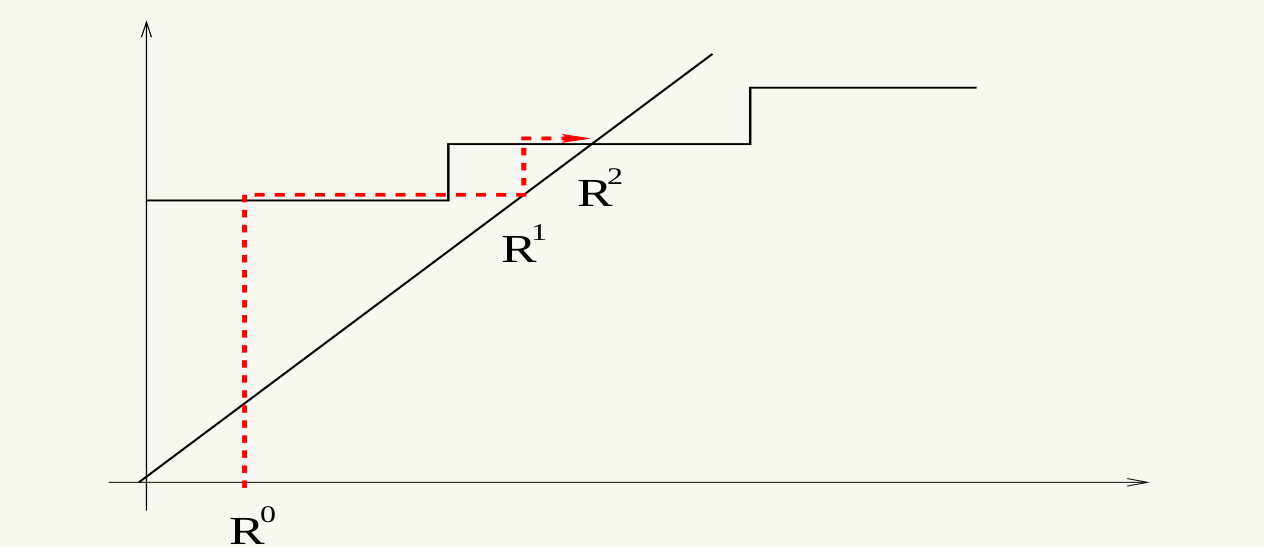
\includegraphics[width=.8\textwidth]{image05}
\end{figure}
The point where the \side{bisector} intersects the stairway, is the solution to the equation. But how one can find such intersection?\\
In terms of algorithms it means that, one have a first guess which is

\begin{itemize}
\item Iterative solution:
\[R_i = \lim_{k\to\infty} R_i^{(k)}\]
where $R_i^{(k)}$ is the worst case response time for $\tau_i$ at step $k$
\item Hence, we can start from a first estimation of the response time:
\[R_{i}^{(0)} = C_i\]
\item Compute the interference in this interval
\[R_{i}^{(1)} = C_i + \sum_{h=1}^{i-1}\ceil{\cfrac{R_{i}^{(0)}}{T_h}} C_h\]
Since all the tasks starts at the same instant (critical instant), I am sure that I would have at least one activation, hence
\[R_i^{(0)} = C_i + \sum_{h=1}^{i-1} C_h\]
\item Repeat the iterative step:
\[R_{i}^{(1)} = C_i + \sum_{h=1}^{i-1}\ceil{\cfrac{R_{i}^{(k-1)}}{T_h}} C_h\]
\item The iteration stops when:
\begin{itemize}
\item $R_i^{(k+1)} = R_i^{(k)}$
\item $R_i^{(k)} > D_i$ (non schedulable)
\end{itemize}
\end{itemize}

This is a standard method to solve non-linear equations in an iterative way. If a solution exists (the system is not overloaded, i.e. total utilisation of the task is below 1), $R_i^{(k)}$ converges to it, otherwise the failing condition avoids infinte iterations.

\subsubsection{Considerations}
\begin{enumerate}
\item The response time analysis is an efficient algorithm
\item In the worst case the number of steps $N$ for the algorithm to converge is exponential
\item depends on the total number of jobs of higher priority tasks in the interval $[0, D_i]$
\[N \propto \sum_{h=1}^{i-1}\ceil{\cfrac{D_h}{T_h}}\]
\item If $s$ is the minimum granularity of the time, then in the worst case 
\[N = \cfrac{D_i}{s}\]
\item However, such worst case is very rare: usually, the number of steps is low.
\end{enumerate}














